\subsection{Idea general del problema}
El ejercicio nos propone diseñar un algoritmo para resolver el siguiente problema: dado un grupo de exploradoras, y el conjunto 
de amigas de cada una de ellas, organizar una ronda de manera tal que exista la menor distancia posible entre cada amistad, es 
decir, minimizar la suma de las distancias entre todos los pares de amigas.\\
La complejidad de la solución debe ser estrictamente menor que O(e$^e$.a$^2$), donde ``e"$ $ es la cantidad de exploradoras en cada grupo, y ``a"$ $ la cantidad de amistades. \\

Algunos ejemplos de posibles datos de entrada del problema son: \\
a bcde;b acde;c abde;d abc;e abc \\
a bcd;b ae;c ad;d ac;e b \\
a fb;b gc;d gc;f agh;e hd \\
x yz \\

Cada línea corresponde a un grupo de exploradoras; y se compone de una exploradora, seguida por una sucesion de amistades
separadas por ``;"$ $. Por ejemplo, en la primer línea, el grupo de exploradoras esta compuesto por ``a"$ $ cuyas amigas son [bcde],
``b"$ $ con [acde], ``c"$ $ con [abde] y por último ``d"$ $ y ``e"$ $ con  [abc]. Asumimos que las amistades son simétricas, es decir, si ``
a"$ $ es amiga de ``b"$ $, entonces ``b"$ $ es amiga de ``a"$ $. Por lo tanto, aunque ocurra que ``x"$ $ este en el conjunto de amigas 
de ``y"$ $, pero ``y"$ $ no este en el de ``x"$ $, debemos interpretarlo como que cada una esta en el grupo de amigas de la otra.  \\

Las salidas que corresponden a los ejemplos recien dados son las siguientes (mismo orden): \\
2 abdce \\
2 abecd \\
3 abgcdehf \\
1 xyz \\

La sucesión de caracteres representa la solución del problema, es decir, la ronda en la que exista la menor distancia posible entre cada 
amistad. El número que está delante, es la máxima distancia que hay entre dos amigas en la ronda solución. Si es que existe mas de una 
ronda óptima, se debe dar la que esté primera alfabéticamente. 

\subsection{Explicación y pseudocódigo}
Para resolver el problema diseñamos un algoritmo que consiste en, dado un grupo de exploradoras, generar todas las rondas 
posibles, e ir almacenando aquella que hasta el momento es la ``mejor"$ $ entre las ya calculadas (con ``mejor"$ $ nos referimos a 
aquella que minimiza la suma de las distancias entre amigas).\\

Para armar las permutaciones, construimos la funcion $permutar$. Mediante esta funcion vamos generando todas las rondas posibles, 
pues cada vez que la llamamos, genera la siguiente permutacion (siguiente en orden alfabético) de la ronda, hasta que ya no hayan 
nuevas. Su algoritmo consiste en buscar el mayor índice k tal que a[k] $<$ a[k+1]; luego buscar el mayor índice i tal que a[k] $<
$ a[i]; swapear a[k] con a[i]; y por último aplicar reverso a partir del elemento k (sin incluirlo) hasta el final de la lista. Entonces, a medida 
que vamos armando las distintas rondas posibles, calculamos la suma de distancias y luego la comparamos con la suma de la que 
tenemos almacenada. Si la suma de la nueva ronda es menor entonces nos guardamos la nueva, pues es ``mejor"$ $ que la que 
teníamos. Caso contrario, pasamos a calcular la siguiente ronda, pues si la suma es mayor esa ronda no nos interesa, y si es igual 
tampoco, porque como las rondas se van calculando en orden alfabetico, entonces la que ya tenemos guardada va a estar primera 
teniendo en cuenta dicho orden. \\

El algoritmo termina una vez que se hayan calculado todas las rondas posibles. La última ronda que quedó guardada va a ser nuestra 
solución. Por otra parte, la máxima distancia entre dos amigas de la ronda, se calcula en simultáneo con la suma de las distancias, y 
siempre la almacenamos junto con la ``mejor"$ $ ronda durante todo el algoritmo. \\

Para entender mejor la idea dejamos el algoritmo en pseudocódigo:\\   
--------------------------------------------------------------------------------------------------------------\\
mejorRonda (dado un conjunto de exploradoras (exp) y sus amistades) \\
$~~~~~~~~$crear int sumaMinima \\
$~~~~~~~~$crear int maxDist \\
$~~~~~~~~$crear Ronda rondaOptima  \\
$~~~~~~~~$ordenar alfabeticamente exp \\
$~~~~~~~~$rondaOptima $\leftarrow$ exp \\
$~~~~~~~~$sumaMinima $\leftarrow$ calcular suma de distancias de rondaOptima  \\
$~~~~~~~~$maxDist $\leftarrow$ calcular maxima distancia entre 2 amigas en rondaOptima \\
$~~~~~~~~$\textbf{mientras} (hay nueva permutacion de exp) \{ \\
$~~~~~~~~~~~~$crear int nuevaSuma $\leftarrow$ calcular suma de distancias de exp  \\
$~~~~~~~~~~~~$crear int nuevaDist $\leftarrow$ calcular maxima distancia entre 2 amigas en exp  \\
$~~~~~~~~~~~~$\textbf{si} (nuevaSuma $<$ sumaMinima) \{ \\
$~~~~~~~~~~~~~~~~$ sumaMinima $\leftarrow$ nuevaSuma \\
$~~~~~~~~~~~~~~~~$ maxDist $\leftarrow$ nuevaDist \\
$~~~~~~~~~~~~~~~~$ rondaOptima $\leftarrow$ exp \\
$~~~~~~~~~~~~$\} \\
$~~~~~~~~$ \} \\
$~~~~~~~~$ exp $\leftarrow$ rondaOptima\\
$~~~~~~~~$ devolver maxDist\\
--------------------------------------------------------------------------------------------------------------\\ \\
El cálculo de la suma de las distancias lo hacemos mediante un algoritmo iterativo que, lo que hace, es recorrer el vector
(que representa a la ronda), y para cada exploradora calcula cuál es la distancia entre ella y cada una de sus amigas (mediante 
otro ciclo interno). Si bien al aplicar $completarAmigas$ se agregan todas las amistades para todas las exploradoras, en el algoritmo se 
tienen en cuenta qué amistades ya fueron sumadas, por lo tanto no vuelven a sumarse (sino estaríamos calculando el doble de la suma 
de distancias). Se repite el procedimiento hasta que el vector se recorre completamente, y así obtenemos la suma de las distancias.
\\
Este algoritmo es correcto pues no dejamos de lado ninguna ronda existente; siempre guardamos la mejor ronda calculada hasta el 
momento; y generamos las rondas en orden alfabético, por lo tanto siempre vamos a obtener la solución deseada.


\subsection{Deducción de la cota de complejidad temporal}

Para la resolución de este ejercicio construimos la clase Ronda en c++. La ronda se representa, en la parte privada de la clase,
mediante un vector$<$char$>$, donde los char representan a las exploradoras y cómo están ubicadas en la ronda. También posee un 
diccionario(utilizamos $<$map$>$ de la STL de c++), donde están asociadas las exploradoras a sus respectivos grupos de amigas. \\
La clase cuenta con el constructor por defecto (ronda vacia) y otro constructor que recibe como parámetros un vector$<$char$>$ y un
vector$<$vector$<$char$>>$; donde el primero representa el conjunto de exploradoras, y el segundo las amigas de cada una (asociadas
por el orden de los vectores). Como el enunciado del ejercicio permite que mismos grupos de exploradoras sean escritos de distintas 
formas (por ejemplo a bc;b ac;c ab también se puede escribir como a b;b c;c ab), construimos la función $completarAmigas$ que se 
encarga de verficar que ninguna amistad esté ausente en la lista de una exploradora, y que estén presentes la totalidad de las 
exploradoras, cada una con su grupo de amigas. Esta función la utilizamos en el constructor, de manera que se almacene en la parte 
privada toda la información completa. \\
A continuación analizamos paso a paso la complejidad temporal de las funciones que implementamos. Para ello, tener en cuenta que 
``e"$ $ representa la cantidad de exploradoras de cada grupo y  ``a"$ $ la cantidad de amistades distintas. \\
La complejidad de $completarAmigas$ es O(e.a) en el peor caso; y el algoritmo consiste en los siguientes pasos (recibe los mismos 
parámetros de entrada que el constructor): \\
\begin{itemize}
\item Recorrer el vector$<$char$>$ que contiene a las exploradoras y por cada exploradora recorrer su grupo de amigas. \\
Costo: 2a = O(a) pues son a amistades y cada una de ellas esta en el grupo de las 2 exploradoras amigas. 
\item Por cada amiga, verificar si está presente en el vector de exploradoras y en caso positivo (si no está presente se agrega, que 
toma O(1)), verificar si la exploradora i está presente en el grupo de dicha amiga(si no está presente se agrega, que 
toma O(1)).  \\
Costo: O(e) pues son dos busquedas lineales con costo O(e) en el peor caso cada una.
\end{itemize}
Finalmente la ecuación de la complejidad del algoritmo es O(e) x O(a) = O(e.a). \\
Otra operación pública de nuestra clase es $sumaDistancias$, que devuelve una dupla de enteros, donde la primer componente 
representa la suma de las distancias entre las exploradoras que son amigas, y la segunda, la mayor distancia entre dos amigas en 
la ronda. A continuación analizamos la complejidad de $sumaDistancias$: 
\begin{itemize}
\item Recorrer el vector$<$char$>$ que contiene a las exploradoras y por cada exploradora buscar su grupo de amigas en el diccionario 
y copiarlo a un vector auxiliar.\\
Costo: O(e$^2$) pues son e exploradoras; buscar en el diccionario es O(log(e))(extraído de cppreference.com) y copiar el vector es O(e) ( 
O(e) + O(log(e)) = O(e) ).
\item Por cada amiga buscamos su posición en la ronda y calculamos la distancia entre ella y la exploradora a la que le corresponde el 
vector de amigas que estamos recorriendo. \\
Costo: O(e.a) pues es buscar su posicion linealmente sobre e elementos (lo hacemos 2.a veces, pero 2.a = O(a) ), y el cálculo de la distancia es O(1).
\end{itemize}
Finalmente la ecuación de la complejidad del algoritmo es O(e$^2$) + O(e.a) = O(e.a) (la cantidad de amistades es mayor o igual que la cantidad de exploradoras, pues cada exploradora tiene al menos una amiga, entonces O(e$^2$) = O(e.a)). \\
\\
Ahora veamos cuál es la complejidad de la función $permutar$:
\begin{itemize}
\item Busqueda lineal del mayor indice k tal que explorers[k] $<$ explorers[k+1]. \\
Costo: O(e).
\item Busqueda lineal del mayor indice i tal que explorers[k] $<$ explorers[i]. \\
Costo: O(e).
\item Swapear explorers[k] y explorers[i]. \\
Costo: O(1).
\item Aplicar reverso a partir del elemento k (sin incluirlo) hasta el final del vector (utilizamos $reverse$ de la STL de c++). \\
Costo: O(e) (extraído de cppreference.com).
\end{itemize}
Finalmente la ecuación de la complejidad del algoritmo es O(e) + O(e) + O(1) + O(e) = O(e).
\\

Otras operaciones que implementamos en la clase Ronda son: 
\begin{itemize}
\item $cambiarOrden$; que cambia las posiciones de las exploradoras en la ronda (lo hace en orden alfabético). Utilizamos la función 
$permutar$, por lo que la complejidad es O(e) en el peor caso.
\item $ordenAlfabetico$; que ordena la ronda alfabéticamente. Para ello usamos la función $sort$ de la STL, con complejidad
O(e.log(e)) (extraido de cppreference.com).
\item $amigasDe$; que devuelve un vector que contiene a las amigas de la exploradora ingresada como parámetro(O(e)).
\item $rondaActual$; que devuelve un esquema de la ronda, mediante un vector (O(e)).
\item $imprimirRonda$ e $imprimirAmistades$; imprimen en consola las ronda y conjunto de amistades respectivamente (utilizadas
principalmente para la prueba y desarollo del trabajo práctico).  
\end{itemize}
Ahora analicemos la complejidad de la principal operación del ejercicio, a la cual llamamos $mejorRonda$, que modifica la Ronda de 
manera
tal que minimice la suma de las distancias entre amigas, y devuelve la maxima distancia entre dos amigas en la ronda solución: 
\begin{itemize}
\item Ordenamos la ronda mediante $ordenAlfabetico$. \\
Costo: O(e.log(e))
\item Hacemos $sumaDistancias$ sobre la ronda ordenada, y guardamos los valores en una dupla de enteros.\\
Costo: O(e.a)
\item Copiamos la ronda actual en una nueva variable. \\
Costo: O(e)
\item Hacemos un ciclo que finaliza cuando hayamos generado todas las permutaciones posibles de la ronda. \\
Costo: O(e!) (cantidad de iteraciones)
\item Por cada iteracion del ciclo realizamos lo siguiente (en el peor de los casos):\\
-$cambiarOrden$ (toma O(e)) \\
-$sumaDistancias$ (toma O(e.a)) \\
-Copiamos una ronda (toma O(e))
\item Copiamos la mejor ronda en la parte privada de la Ronda. \\
Costo: O(e)
\item Copiamos un entero a una nueva variable. \\
Costo: O(1)
\end{itemize}
Entonces, la complejidad de la función es:\\ \\
$\underbrace{$O(e.log(e)) + O(e.a)+ O(e)$}_{O(e.a)\;}$ + $\underbrace{$O(e!) x \big( O(e) + O(e.a) + O(e) \big)$ }_{O(e!.e.a) \;}$+
$\underbrace {$O(e) + O(1)$}_{O(e)\;}$ \\ \\
O(e.a) + O(e!.e.a) + O(e) = O(e!.e.a) \\
\\
Ahora, demostraremos que la complejidad de nuestro algoritmo cumple con la cota dada: \\
\\
Aclaraciones: si bien $completarAmigas$ y $mejorRonda$ son dos operaciones distintas en nuestro proyecto, ambas forman parte de la
solución del ejercicio, por lo tanto para demostrar que cumplimos con la cota dada en el enunciado, tenemos en cuenta las complejidades 
de las dos operaciones (de todas formas, la complejidad teórica no cambia).\\
\\
O(e!.e.a) + O(e.a) = O(e!.e.a) \\ 
\\
Hechas las aclaraciones, comenzamos con la demostración:
\begin{itemize}
\item Queremos ver que O(e!.e.a) $\subseteq$ O(e$^e$.a$^2$)
\item Para demostrarlo, probemos que e!.e.a $\in$ O(e$^e$.a$^2$) (pues si f $\in$ O(g) $\Rightarrow$ O(f) $\subseteq$ O(g) )
\item Por definicion de O; e!.e.a $\in$ O(e$^e$.a$^2$) $\Leftrightarrow$ $\exists$ $n_{0}$ $>$ 0,  c $>$ 0  $/$ $\forall$ (n $>$ $n_
{0}$) e!.e.a $\leq$ c.e$^e$.a$^2$ 
\item Entonces, veamos que e!.e.a $\leq$ c.e$^e$.a$^2$  $\forall$ (n $>$ $n_{0}$)
\item Y para probar lo anterior basta con ver que e!.e.a $\leq$ c.e$^e$ $\forall$ (n $>$ $n_{0}$): \\
e! = $\underbrace{$1.2.3........e$}_{e \ productos\;}$ $\leq$ $\underbrace{$e.e.e........e$}_{e \ productos\;}$ = e$^e$ \\ \\
Sabemos que la anterior desigualdad es cierta, pues todos los factores de la multiplicación del lado izquierdo son menores o iguales que 
los del lado derecho. \\
Entonces veamos si vale lo siguiente: e!.e.a  = $\underbrace{$1.2.3........e$}_{e \ productos\;}$ .  e.a $\leq$ c. $\underbrace{$e.e.e........e$}_{e \ productos\;}$ = c.e$^e$  \\
¡Si, vale! Pues si acomodamos un poco los productos, acotamos superiormente e.a por e$^2$ (pues la maxima cantidad de amistades posibles es $\sum_{i=1}^{e-1} i$ = $\frac{(e-1).e}{2}$ $\leq$ e$^2$ ), y tomamos c = 1.2.3 = 6 nos queda que:\\
\\
e!.e.e$^2$ = 6. $\underbrace{$4.5.6........e.e.e.e$}_{e \ productos\;}$ $\leq$ 6. $\underbrace{$e.e.e........e$}_{e \ productos\;}$ = c.e$^e$ \\
Y con el mismo razonamiento de antes (todos los factores de la multiplicación del lado izquierdo son menores o iguales que 
los del lado derecho) concluimos que vale la desigualdad.
Entonces e!.e.a $\in$ O(e$^e$.a$^2$) $\Rightarrow$ O(e!.e.a) $\subseteq$ O(e$^e$.a$^2$), y concluimos que nuestro algoritmo respeta
la cota dada por el enunciado.


\\

\subsection{Experimentación}

Para analizar el comportamiento de nuestro algoritmo, evaluamos su desempeño mediante varios casos de test, que nos permitieron realizar los siguientes gráficos y conclusiones. Pusimos pocos valores (de tamaño de entrada) en el gráfico, pues la complejidad y el tiempo de ejecución del algoritmo crece muy rápidamente, por lo que no podemos testearlo con casos mas grandes. 

\begin{figure}[H] 
\begin{center}

\minipage{0.8\textwidth}
  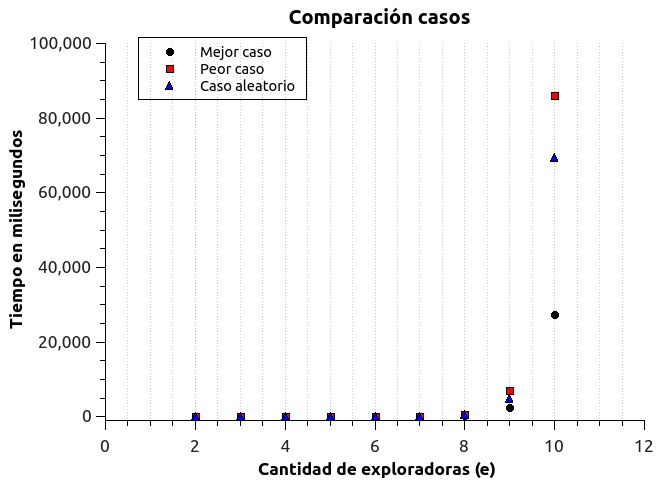
\includegraphics[width=\linewidth]{../graficos/ej3/ComparacionCasos.png}
  \caption{{\small Comparación de los mejores y peores casos para cada tamaño de entrada. También incluimos casos aleatorios.}} \label{asd}
\endminipage

\end{center}
\end{figure} 

Los mejores casos son aquellos en los que las exploradoras tienen solo una amiga cada una, pues a la hora de calcular las distancias, hay menos amistades que sumar a la suma total. Al contrario, los peores casos son aquellos en los que todas las exploradoras son amigas con todas. Damos un ejemplo de peor y mejor caso para un ronda de 6 exploradoras: \\
a bcdef (mejor caso) \\
a bcdef;b cdef;c def;d ef;e f (peor caso) \\
Las instancias de mejores y peores casos las generamos manualmente, mientras que para las de casos aleatorios hicimos un generador (ver generador.cpp)


\begin{figure}[H] 
\begin{center}

\minipage{0.8\textwidth}
  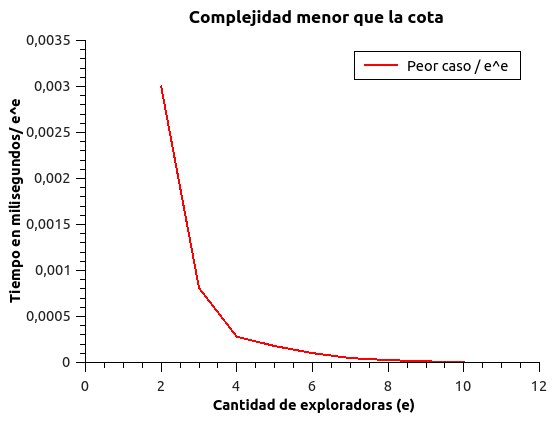
\includegraphics[width=\linewidth]{../graficos/ej3/Complejidad.png}
  \caption{{\small Complejidad de nuestro algoritmo acotada por la del enunciado.}} \label{asd}
\endminipage

\end{center}
\end{figure}

En este gráfico dividimos los tiempos de los peores casos por e$^e$ y como la curva tiende a 0, concluimos que la complejidad de nuestro algoritmo es
menor que e$^e$.\\

Aclaración: en los archivos y carpetas de código se pueden ver muchos ejemplos para testeo.




